\section{Success criteria}

Referring to the~\nameref{ch:proposal}, I met all success criteria of the project


\begin{todolist}
    \item[\done] Implemented the experimental framework (\graffs) to automate experiments of robustness of graph metrics
    \item[\done] Completed statistical analysis and compared results to The Paper
    \item[\done] Extended the idea from The Paper to unscored networks, and deduced empirical observations about graph metrics on interesting unscored datasets
\end{todolist}

For the evaluation of \graffs, I designed the following experiments:
\begin{description}
    \item[\texttt{reproduce}] focuses on reproducing some results from The Paper, following the setup from The Paper as closely as possible
    \item[\texttt{random-edges}] validates whether random edge deletion is a suitable graph generation method, by applying the same pipeline as in \texttt{repr} just with random edge deletion
    \item[\texttt{unscored}] applies the random edge deletion method to new, unscored, datasets
\end{description}

In analyses in the following sections, the protein network datasets \texttt{pvivax}, \texttt{ecoli}, \texttt{yeast} are the exact datasets that were used in The Paper\footnote{The datasets are available at \url{https://github.com/lbozhilova/measuring_rank_robustness}}.
They originate from the STRING database, but the database changes over time, so to validate \graffs by reproducing the results I preferred using the same datasets over their new version.


\section{Validation against The Paper}

One of the added values of \graffs is the ability to experiment with \textsl{unscored} graphs.
However, in order to validate whether the results produced by \graffs are legit, I first constructed and ran a \texttt{reproduce} experiment trying to reproduce results from The Paper, by linearly thresholding 3 scored protein interaction networks in the same way as The Paper.

The \texttt{reproduce} experiment with the \texttt{thMedHigh} generator (producing 31 graphs at linearly spaced thresholds between 0.60 and 0.90 confidence values) were set up in the following way:
% @formatter:off
\begin{lstlisting}[language=bash]
graffs dataset download-demos
graffs generator create --name thMedHigh --method threshold-linear --params 600,900 -n 31 --seed 7
graffs experiment create --name reproduce --datasets pvivax,ecoli,yeast --generator thMedHigh --metrics Betweenness,Degree,Ego1Edges,Ego2Nodes,LocalClustering,PageRank,Redundancy --robustnessMeasures RankIdentifiability,RankInstability,RankContinuity
graffs experiment run --name reproduce
\end{lstlisting}
% @formatter:on

As for the set of metrics, I evaluated all that were also evaluated in The Paper, apart from Closeness and Harmonic centrality (Definitions~\ref{def:closeness_centrality} and~\ref{def:harmonic_centrality}).
These two depend on the all pair shortest paths algorithm with time complexity $O({\left\lvert V \right\rvert}^3)$ that would take unreasonable amount of time to compute on large graphs. (\todo{evaluating Closeness on one graph takes XY minutes\ldots})

\begin{figure}
    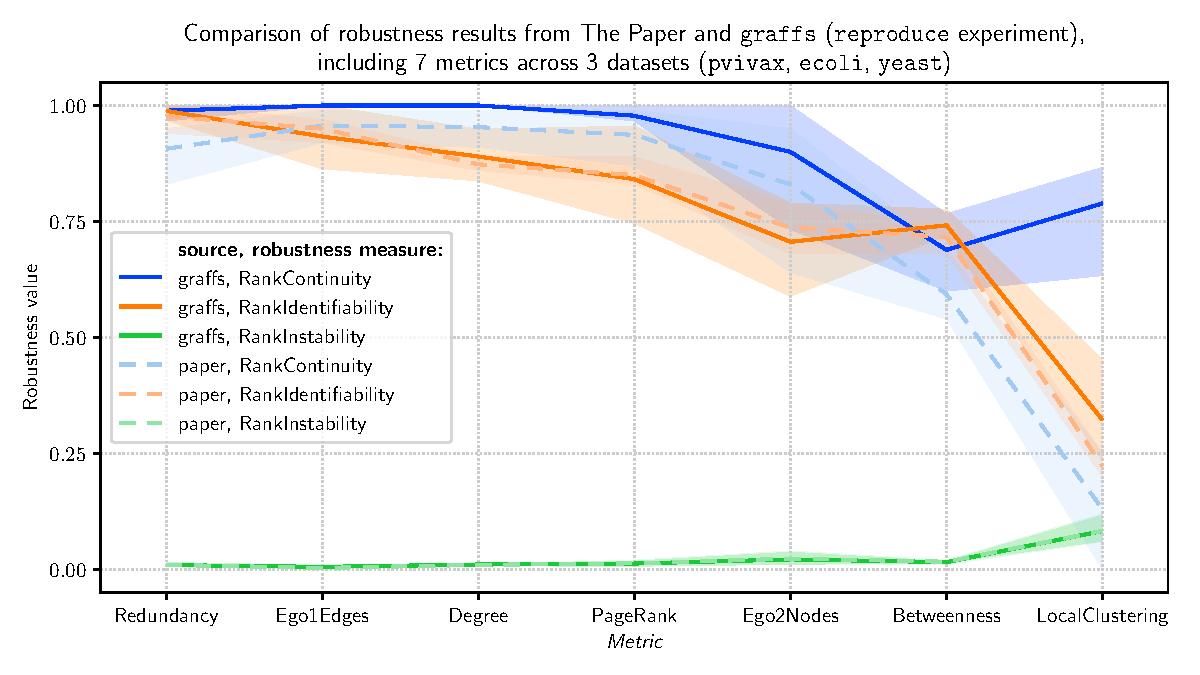
\includegraphics[width=\linewidth]{plot_reproduction.pdf}
    \caption{Comparison of results from The Paper and \graffs.
    Each color corresponds to one robustness measure, with thin lines inside each band showing robustness of individual datasets, and the thick line showing the average robustness across the 3 datasets.
    Solid and dashed bands correspond to results obtained by \graffs and The Paper, respectively.}
    \label{fig:plot_reproduction}
    \footnotesize
    \begin{flushleft}
        Note that high values of RankContinuity and RankIdentifiability mean high \textsl{robustness}, whereas high values of RankInstability mean low \textsl{robustness}.
        Metrics are sorted from left to right by their decreasing combined robustness.
    \end{flushleft}
\end{figure}


\autoref{fig:plot_reproduction} demonstrates that \graffs is able to identify similar robustness properties of metrics as in The Paper.
The Paper identifies metrics \texttt{Ego1Edges}, \texttt{Redundancy}, \texttt{Ego2Nodes}, \texttt{Degree} as very stable (i.e. robust).
Those have reported RankContinuity and RankIdentifiability values above $0.75$ on almost all evaluations on the 3 datasets, and RankInstability below $\sim 0.1$.
\graffs also reports these metrics as relatively stable, although the RankIdentifiability value is lower in general.

On the other hand, \texttt{Betweenness} and \texttt{LocalClustering} are considered unstable by The Paper (RankContinuity and RankIdentifiability significantly dropped while RankInstability increased), and the results from \graffs copy the behaviour.
Although the RankContinuity values of \texttt{LocalClustering} are not as low as reported by The Paper, one can definitely conclude that these two metrics are equally identified as less robust by \graffs.

The robustness values from The Paper and \graffs should not be compared directly as there are many implementation details that make the numerical values vary between implementations.
For example, when ranking nodes according to a metric, The Paper resolved ties randomly for each perturbed graph (which already leads to fluctuations in rankings), and my implementation resolves ties arbitrarily but predictably and constantly across all perturbed graphs of a dataset, with the purpose to improve reliability of robustness measures.
The Paper also randomly resolved ties when calculating the overall ranking (Definition~\ref{def:overall_ranking}).
Furthermore, there are other nuances that may cause these variations, such as $\alpha,k$ coefficients used for $k$-similarity and $\alpha$-relaxed $k$-similarity (definitions~\ref{def:k_similarity},~\ref{def:alpha_relaxed_k_similarity}), definitions of graph metrics in special cases (such as for isolated nodes), and floating-point arithmetic.

For further thought, we can also consider variance of robustness measures to conclude that \texttt{Redundancy} (a stable metric) was assessed with variance close to zero, whereas the RankContinuity and RankIdentifiability measures of the \texttt{Ego2Nodes} metric led to diverse values across the 3 datasets.

\todo{add timings}
%Generate graphs            : 51s
%Evaluate metrics - run     : 38m 46s
%Robustness - compute       : 10s


\section{Validation of random edge deletion}

Randomly deleting a small subset of edges allows us to evaluate robustness of metrics on unscored graphs.
The purpose of the \texttt{random-edges} experiment is to justify reliability and accuracy of this approach.

I set the $\alpha$ parameter (proportion of edges to delete; see \autoref{eq:edge_removing_generator}) equal to $4\%$.
This is following

The experiment was set up in the following way:
% @formatter:off
\begin{lstlisting}[language=bash]
graffs dataset download-demos
graffs generator create --name thMedHigh --method threshold-linear --params 600,900 -n 31 --seed 7
graffs experiment create --name reproduce --datasets pvivax,ecoli,yeast --generator thMedHigh --metrics Betweenness,Degree,Ego1Edges,Ego2Nodes,LocalClustering,PageRank,Redundancy --robustnessMeasures RankIdentifiability,RankInstability,RankContinuity
graffs experiment run --name reproduce
\end{lstlisting}
% @formatter:on


\section{Reliability of \graffs}

- why is~\nameref{sec:randomly_removing_edges} as good as thresholding?
maybe apply Randomly removing edges to scored networks and see the difference of robustness


\section{Reproducing results}


\section{Extending to further datasets}


\section{(Predicting metric stability)}


\section{Releasing \graffs}

\subsection{Licensing}
